\documentclass[tikz,border=0pt]{standalone}
\usepackage[utf8]{inputenc}
\usepackage[T1]{fontenc}
\usepackage{lmodern}
\usepackage{amsmath,amssymb}
\usetikzlibrary{arrows.meta,positioning,fit,calc,backgrounds,shapes.geometric,decorations.pathreplacing}
\definecolor{navy}{HTML}{163A5F}
\definecolor{blue}{HTML}{2C6EAF}
\definecolor{lightblue}{HTML}{EAF2F8}
\definecolor{midblue}{HTML}{CFE1F2}
\definecolor{graytext}{HTML}{4A5560}
\definecolor{lightgray}{HTML}{F4F6F8}
\definecolor{green}{HTML}{3C8D73}
\definecolor{lightgreen}{HTML}{E8F5EF}
\definecolor{red}{HTML}{B24A4A}
\definecolor{lightred}{HTML}{FBEDEE}
\tikzset{
  title/.style={font=\sffamily\bfseries\fontsize{18}{20}\selectfont,text=navy,anchor=west},
  subtitle/.style={font=\sffamily\bfseries\fontsize{11}{13}\selectfont,text=navy},
  body/.style={font=\sffamily\fontsize{9.2}{11}\selectfont,text=graytext,align=left},
  small/.style={font=\sffamily\fontsize{8}{9.4}\selectfont,text=graytext,align=left},
  tinylabel/.style={font=\sffamily\fontsize{7.2}{8.4}\selectfont,text=graytext},
  panel/.style={rounded corners=3pt,draw=midblue,fill=white,line width=0.6pt},
  box/.style={rounded corners=2pt,draw=midblue,fill=lightblue,line width=0.6pt},
  worker/.style={rounded corners=2pt,draw=blue,dashed,line width=0.7pt,fill=white},
  task/.style={rounded corners=2pt,draw=blue,fill=lightblue,minimum width=0.85cm,minimum height=0.55cm,font=\sffamily\bfseries\small,text=navy},
  file/.style={draw=blue,fill=white,minimum width=0.55cm,minimum height=0.42cm,font=\sffamily\small,text=navy},
  arr/.style={-{Stealth[length=2.4mm,width=1.8mm]},draw=blue,line width=0.9pt},
  arrthin/.style={-{Stealth[length=2mm,width=1.5mm]},draw=blue,line width=0.7pt},
  arrred/.style={-{Stealth[length=2mm,width=1.5mm]},draw=red,dashed,line width=0.8pt},
  arrgreen/.style={-{Stealth[length=2mm,width=1.5mm]},draw=green,dotted,line width=1pt}
}
\begin{document}

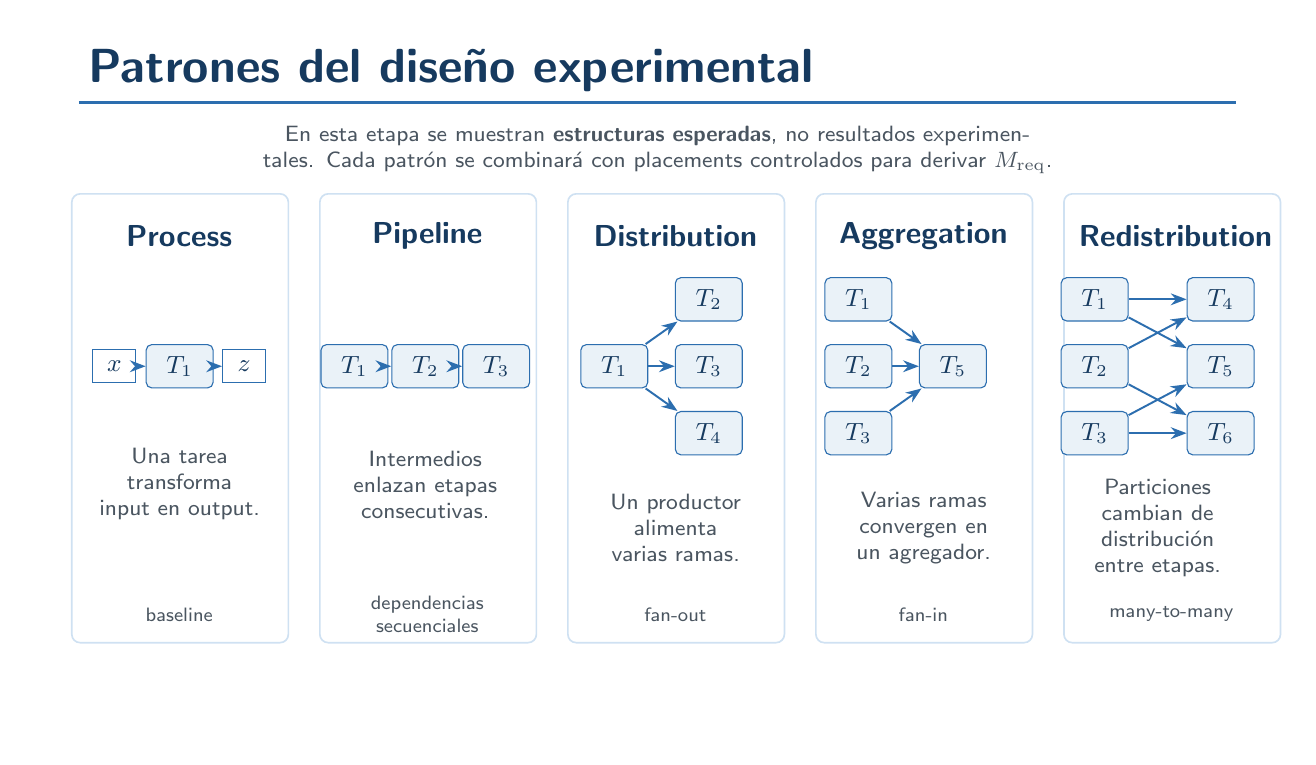
\begin{tikzpicture}[x=1cm,y=1cm]
\path[use as bounding box] (0,0) rectangle (16,9);
\node[title] at (0.65,8.45) {Patrones del diseño experimental};
\draw[blue,line width=1pt] (0.65,8.05)--(15.35,8.05);
\node[small,text width=14.2cm,align=center] at (8,7.45) {En esta etapa se muestran \textbf{estructuras esperadas}, no resultados experimentales. Cada patrón se combinará con placements controlados para derivar $M_{\mathrm{req}}$.};

% panels positions
\foreach \x/\ttl/\cap in {0.55/{Process}/{baseline},3.7/{Pipeline}/{dependencias secuenciales},6.85/{Distribution}/{fan-out},10.0/{Aggregation}/{fan-in},13.15/{Redistribution}/{many-to-many}}{
\node[panel,minimum width=2.75cm,minimum height=5.7cm,anchor=north west] at (\x,6.9) {};
\node[subtitle,text width=2.35cm,align=center] at (\x+1.375,6.35) {\ttl};
\node[tinylabel,text width=2.3cm,align=center] at (\x+1.375,1.55) {\cap};
}
% process
\node[file] (pfin) at (1.1,4.7) {$x$}; \node[task] (pt1) at (1.93,4.7) {$T_1$}; \node[file] (pfout) at (2.75,4.7) {$z$};
\draw[arrthin] (pfin)--(pt1); \draw[arrthin] (pt1)--(pfout);
\node[small,text width=2.2cm,align=center] at (1.93,3.2) {Una tarea transforma input en output.};
% pipeline
\node[task] (q1) at (4.15,4.7) {$T_1$}; \node[task] (q2) at (5.05,4.7) {$T_2$}; \node[task] (q3) at (5.95,4.7) {$T_3$};
\draw[arrthin] (q1)--(q2); \draw[arrthin] (q2)--(q3);
\node[small,text width=2.2cm,align=center] at (5.05,3.2) {Intermedios enlazan etapas consecutivas.};
% distribution
\node[task] (d1) at (7.45,4.7) {$T_1$}; \node[task] (d2) at (8.65,5.55) {$T_2$}; \node[task] (d3) at (8.65,4.7) {$T_3$}; \node[task] (d4) at (8.65,3.85) {$T_4$};
\draw[arrthin] (d1)--(d2); \draw[arrthin] (d1)--(d3); \draw[arrthin] (d1)--(d4);
\node[small,text width=2.2cm,align=center] at (8.23,2.65) {Un productor alimenta varias ramas.};
% aggregation
\node[task] (a1) at (10.55,5.55) {$T_1$}; \node[task] (a2) at (10.55,4.7) {$T_2$}; \node[task] (a3) at (10.55,3.85) {$T_3$}; \node[task] (a5) at (11.75,4.7) {$T_5$};
\draw[arrthin] (a1)--(a5); \draw[arrthin] (a2)--(a5); \draw[arrthin] (a3)--(a5);
\node[small,text width=2.2cm,align=center] at (11.38,2.65) {Varias ramas convergen en un agregador.};
% redistribution
\node[task] (r1) at (13.55,5.55) {$T_1$}; \node[task] (r2) at (13.55,4.7) {$T_2$}; \node[task] (r3) at (13.55,3.85) {$T_3$};
\node[task] (r4) at (15.15,5.55) {$T_4$}; \node[task] (r5) at (15.15,4.7) {$T_5$}; \node[task] (r6) at (15.15,3.85) {$T_6$};
\draw[arrthin] (r1)--(r4); \draw[arrthin] (r1)--(r5); \draw[arrthin] (r2)--(r4); \draw[arrthin] (r2)--(r6); \draw[arrthin] (r3)--(r5); \draw[arrthin] (r3)--(r6);
\node[small,text width=2.2cm,align=center] at (14.35,2.65) {Particiones cambian de distribución entre etapas.};
\end{tikzpicture}
\end{document}
